\chapter{Introduction}%
\label{ch:introduction}%
Using \verb|\parencite| produces a reference in parentheses, for example \parencite{bishopPatternRecognitionMachine2006}. In contrast, using \verb|\textcite| produces a reference without parentheses, for example \textcite{rumelhartLearningRepresentationsBackpropagating1986}. 	

\lipsum%
%
\section{Motivation}%
\label{sec:motivation}%
\lipsum%
\begin{figure}
	\centering
	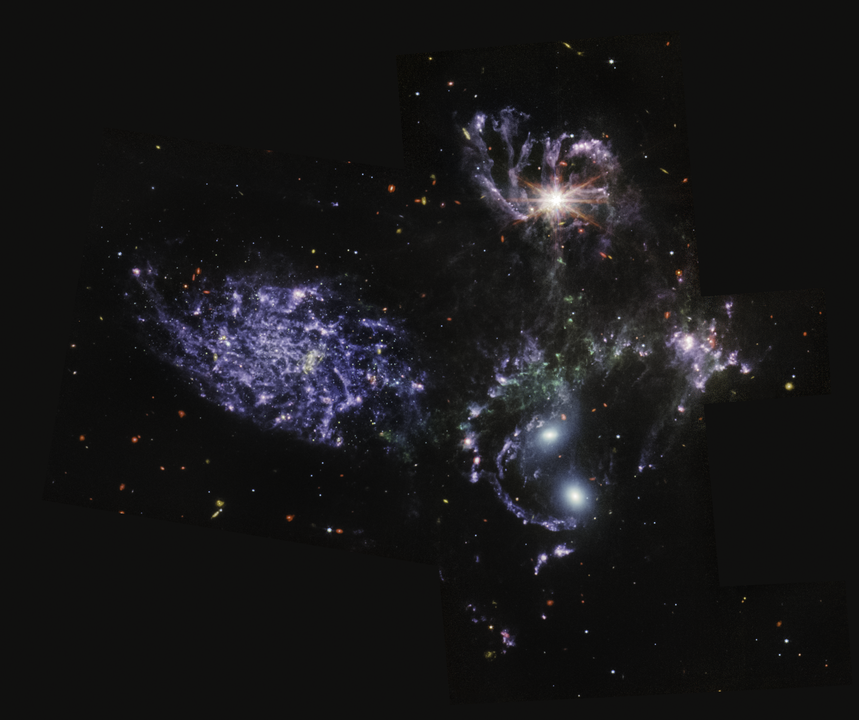
\includegraphics{jamesWebb}
	\caption[James Webb Stephan's Quintet]{Image of the Stephan's Quintet recorded by the James Webb telescope}
	\label{fig:jamesWebb}	
\end{figure}
%
\section{Objectives}%
\label{sec:objectives}%
\lipsum%
%
\section{csquotes package}%
\label{sec:csquotes}
With \verb|\enquote| a simple quotation can be displayed inline, for example \enquote{A short quote.} In contrast, using \verb|\blockquote| will display larger quotes as a separate block: \blockquote[\cite{bishopPatternRecognitionMachine2006}, p.~1]{The problem of searching for patterns in data is a fundamental one and has a long and successful history. For instance, the extensive astronomical observations of Tycho Brahe in the 16th century allowed Johannes Kepler to discover the empirical laws of planetary motion, which in turn provided a springboard for the development of classical mechanics. Similarly, the discovery of regularities in atomic spectra played a key role in the development and verification of quantum physics in the early twentieth century. The field of pattern recognition is concerned with the automatic discovery of regularities in data through the use of computer algorithms and with the use of these regularities to take actions such as classifying the data into different categories.}
%
\section{siunitx package}%
\label{sec:siunitx}
A quantity can be displayed using \verb|\qty[<option>]{<number>}{<unit>}|, for example \qty{9.81}{\meter\per\second\squared}. The units can be formatted differently by setting a specific option. For example, by adding the option \verb|per-mode = symbol|, the quantity is displayed as \qty[per-mode = symbol]{9.81}{\meter\per\second\squared}. In contrast, by adding the option \verb|per-mode = faraction|, the quantity is displayed as \qty[per-mode = fraction]{9.81}{\meter\per\second\squared}.

Other features include the \verb|\qtylist{<numbers>}{<units>}| command for a list of quantities, such as \qtylist{1; 2; 3}{\meter}, and the \verb|\qtyrange{<start>}{<stop>}{<units>}| command for a range of quantities producing \qtyrange{1}{4}{\meter}.
%
\section{cleveref package}%
\label{sec:cleveref}
With the cleveref package, cross-referencing to \cref{fig:jamesWebb} or \cref{ch:introduction}, for example, becomes more convenient. The reference is integrated using the \verb|\cref{<label>}| command. When the number of the referenced object changes, cleveref will notice that and handle the update of all references. 

Note, that the object that should be cross-referenced needs a label. For example, \cref{fig:jamesWebb} has the label \verb|\label{fig:jamesWebb}|.

If the referenced objects should be capitalized, the \verb|\Cref{<label>}| command can be used. \Cref{fig:jamesWebb}, for example, is at the beginning of a sentence and should be capitalized. 
%
\section{enumitem package}%
\label{sec:enumitem}
With the enumitem package, custom labels for lists are enabled. For example:
\begin{enumerate}[leftmargin=*, align=left,start=1,label={\bfseries L\arabic*}]%
	\item \lipsum[0-1]
	\item \lipsum[0-1]
	\item \lipsum[0-1]
\end{enumerate}
%
\section{bib2gls and glossaries-extra packages}%
\label{sec:gls}
With the \verb|\gls{<label>}| command, an abbreviation, a symbol or an example notation can be displayed. For example, the first time derivative can be denoted as \gls{x_dot} and acronyms such as \gls{ml} or \gls{dl} can be handled automatically. When \gls{ml} is called for the second time, only its acronym is displayed. Also, plural terms are possible with the \verb|\glspl{<label>}| command, so that several \glspl{fft} are displayed in plural. Exemplary use for notations and symbols could be the following: the determinant of matrix $X$ can be denoted as \gls{determinant} and the angular velocity can be denoted as \gls{omega}. 

\section{Integrating vector graphics}%
\label{sec:svg}
\lipsum[0-3]
\begin{figure}
	\centering
	\includesvg{plot}
	\caption{A sample vector graphic}
	\label{fig:plot}
\end{figure} 	
